\section{Introduction}
\label{sec:intro}

Text-to-image diffusion models learn a denoising process conditioned on natural-language descriptions, predicting how to recover a clean image from noise~\cite{NEURIPS2020_4c5bcfec,Rombach_2022_CVPR,pmlr-v235-esser24a,flux2024}.
At inference time, this learned model progressively transforms random noise into images that reflect the objects, attributes, and composition specified by a prompt.
The generative capabilities that models acquire from large-scale datasets also raise concerns:
they can generate not-safe-for-work (NSFW) content, reproduce recognizable IP characters, or imitate the painting style of a particular artist~\cite{Schramowski_2023_CVPR,Gandikota_2023_ICCV,Cai_2026_CVPR},
posing risks of harmful content exposure, intellectual property disputes, and economic or reputational harm to creators.
To mitigate these issues, concept erasure has been proposed to selectively suppress designated target concepts while preserving the model's generative capability for unrelated content~\cite{Gandikota_2023_ICCV}.

Existing concept erasure methods typically intervene in either model parameters or the generation process.
Weight-editing approaches~\cite{Gandikota_2023_ICCV,Gandikota_2024_WACV,Kumari_2023_ICCV,pmlr-v267-gao25j} update model parameters to reduce the likelihood of generating a target concept; however, an update intended for one specific concept often bleeds into unrelated content, causing collateral damage.
Inference-time methods~\cite{Schramowski_2023_CVPR,pan2025safecfg,shin2025promptbasedsafetyguidanceineffective,jain2026rethinkingnegativepromptingconcept} offer an alternative by steering the sampling trajectory while keeping model weights fixed,
yet applying the same suppression condition indiscriminately can still alter generations for inputs that require no such intervention.
Among inference-time approaches, negative prompting provides a flexible interface for controlling generation through the model's conditioning inputs.
Within classifier-free guidance~\cite{CFG}, contrasting a negative prompt against the user's prompt steers generation away from unwanted content~\cite{jain2026rethinkingnegativepromptingconcept}.
Although a natural-language description can specify what to avoid, directly using such text as a negative prompt often fails to effectively suppress the target concept, as shown in \cref{fig:negative_prompt}.
TraSCE~\cite{jain2026rethinkingnegativepromptingconcept} demonstrates that naive negative prompting can fail on adversarial inputs when positive and negative predictions collapse together.
These limitations motivate learning an effective negative prompt while selectively deciding when to activate it, as illustrated in \cref{fig:das_teaser}.

\begin{figure}[t]
    \centering
    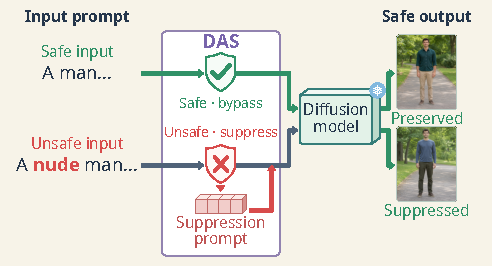
\includegraphics[width=\columnwidth]{figures/teaser-svg.pdf}
    \caption{\textbf{An illustration of Detect and Suppress (DAS).} Safe inputs follow standard generation. When a detection prompt identifies a target concept, its paired suppression prompt is activated in the negative branch of the frozen diffusion model.}
    \label{fig:das_teaser}
\end{figure}

% At a shared noisy state, the original input and the learned negative condition jointly determine the guided prediction, which is explicitly optimized to match the safe reference prediction.
Recognizing that detecting target concepts in a user's prompt and suppressing them serve fundamentally different roles—one classifies inputs by semantic similarity, while the other reshapes generative trajectories—we introduce a safe generation framework: \textbf{Detect and Suppress (DAS)}.
Our framework assigns each target concept a pair of independently learned prompt embeddings tailored to these complementary objectives.
Specifically, the \emph{detection prompt} establishes a concept-specific reference in the text embedding space, using similarity matching to determine whether the target concept is present in the input.
This detection outcome subsequently governs whether to activate the corresponding \emph{suppression prompt}, which acts as a tailored negative condition during generation.
While these two prompts are semantically paired by the target concept, their separate learning objectives allow each representation to specialize without compromise.

To achieve this specialization, we train the detection prompt via text discrimination and visual reconstruction, while optimizing the suppression prompt by aligning the guided predictions of inputs containing the target concept with those obtained from a safe reference prompt.
This training objective endows the suppression prompt with direct control over the sampling updates, forging a clear link between the learned condition and the desired safe behavior while keeping both the text encoders and the generative model entirely frozen.
At inference time, detection is performed just once prior to sampling: an activated suppression prompt is injected as the negative condition, whereas inputs that bypass detection retain their original sampling pathways.

\begin{figure}[t]
    \centering
    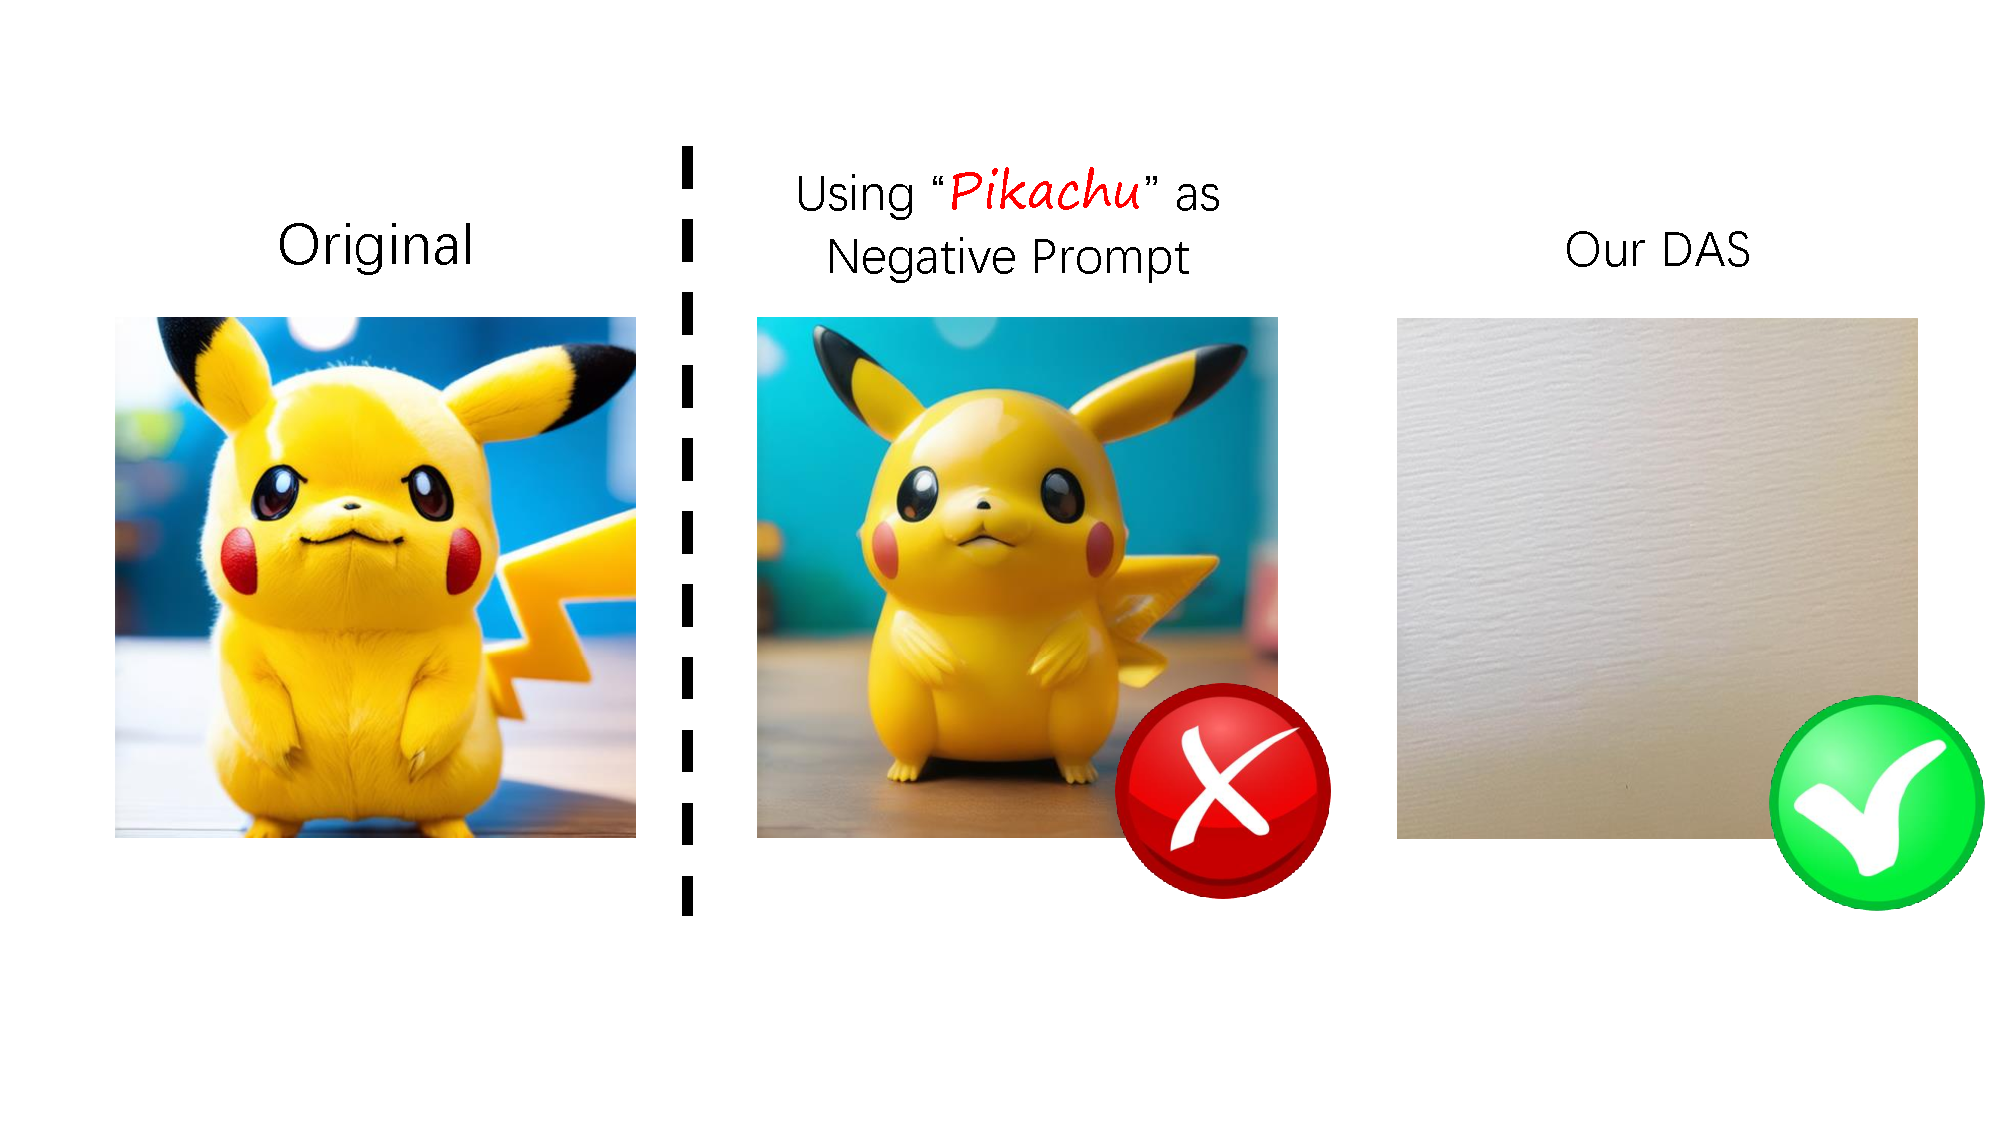
\includegraphics[width=\columnwidth,trim=45bp 87bp 0bp 60bp,clip]{figures/negative_prompt.pdf}
    \caption{\textbf{Concept text can fail as a negative prompt.} The original output (left) and the output using ``Pikachu'' as the negative prompt (middle) both contain the character ``Pikachu'', whereas DAS suppresses it (right).}
    \label{fig:negative_prompt}
\end{figure}

We evaluate DAS on the Diffusion Transformer (DiT)-based Stable Diffusion 3.5 Medium across NSFW suppression, IP character erasure, artistic style erasure, and object erasure, with single- and multiple-concept settings for IP characters and objects.
Across these tasks, DAS achieves stronger target suppression than the compared baselines while preserving unrelated concepts and benign generation.
These findings validate the versatility and robustness of DAS, confirming its efficacy across a diverse range of concept erasure tasks.

Our contributions are as follows:
\begin{itemize}
    \item We formulate selective concept suppression through learned prompt pairs that separate the decision to intervene from the condition used to control generation.
    \item We develop separate objectives for learning a detection prompt from concept discrimination and a suppression prompt from safe reference predictions within a frozen model.
    \item Extensive experiments on NSFW content, IP characters, artistic styles, and objects show that our method achieves superior performance in suppressing target concepts while preserving benign generation.
\end{itemize}
